\documentclass{beamer}

\mode<presentation>
{
	\usetheme{Madrid}
	\usecolortheme{orchid}
}

\usepackage{setspace}

\title{Alias Analysis for Object-Oriented Programs}
\subtitle{\textit{M. Sridharan, S. Chandra, J. Dolby, S. J. Fink, and E. Yahav} \newline\newline \large{Paper Review}}
\institute{Nazarbayev University}
\author{Adilet Zhaxybay}
\subject{Theoretical Computer Science}
\date{}

% Delete this, if you do not want the table of contents to pop up at
% the beginning of each subsection:
\AtBeginSection[]
{
  \begin{frame}<beamer>{Outline}
    \tableofcontents[currentsection,currentsubsection]
  \end{frame}
}
\AtBeginSubsection[]
{
  \begin{frame}<beamer>{Outline}
    \tableofcontents[currentsection,currentsubsection]
  \end{frame}
}

\begin{document}

\begin{frame}
	\titlepage
\end{frame}

\begin{frame}{Outline}
  \tableofcontents
  % You might wish to add the option [pausesections]
\end{frame}

\section{Introduction}

\subsection{Introduction}

\begin{frame}{Alias Analysis}
	\begin{block}{Aliases}
		Two pointers said to be \textit{aliases} if they point to the same location
	\end{block}
	\pause
	\begin{block}{Alias Analysis}
		Analysis which determines which pointers may or must be aliases
	\end{block}	
\end{frame}

\begin{frame}{Example of Aliases}
	\begin{block}{Example in C}
		int * x, y, z;
		\newline
		x = malloc(sizeof(int)); 
		\newline
		y = x; // x and y are aliases now
		\newline
		z = malloc(sizeof(int));  // x and z are not aliases
	\end{block}
\end{frame}

\begin{frame}{Paper Structure}
	\begin{block}{Origin}
		Work by Sridharan et al. gives a high-level survey of the alias-analiysis techniques that authors 
		have found most-useful during a years-long effort developing industrial-strength analyses for Java
		programs.
	\end{block}
	\pause
	\begin{block}{}
		Published in 2013 in `Lecture Notes in Computer Science`
	\end{block}
	\pause
	\begin{block}{}
		It is \textit{not} an exhaustive survey of alias analysis.
	\end{block}
	\pause
	\begin{block}{Challenges}
		Treats alias analysis as a constrant tradeoff between \textit{scalability} (adaptation to large
		 programs) and \textit{precision} (accuracy of analysis).
	\end{block}
\end{frame}

\begin{frame}{Paper Focus}
	\begin{block}{Focus}
		Paper focuses on two main techniques:
	\end{block}
	\pause
	\begin{block}{}
		Points-to analysis --- analysis, that can be used to determine \textit{may-alias} information,
		i.e., whether it is possible for two pointers to be aliased during program execution.
	\end{block}
	\pause
	\begin{block}{}
		Access-path tracking --- provides \textit{must-alias} information, i.e., whether two pointers must be
		aliased at some program point.
	\end{block}
	\pause
	\begin{block}{Java}
		Additionally paper aims to explain particlar challenges for modern Java programs.
	\end{block}
\end{frame}

\subsection{Motivating Analyses}

\begin{frame}{Possible Errors}
	\begin{block}{Memory leak}
		int * x = malloc(sizeof(int));
		\newline
		x = malloc(sizeof(int));
	\end{block}
	\pause
	\begin{block}{Invalid memory access}
		int * x = malloc(sizeof(int));
		\newline
		int * y = x; 
		\newline
		free x;
		\newline
		free y;
	\end{block}	
\end{frame}

\begin{frame}{More Sophisticated Example}
	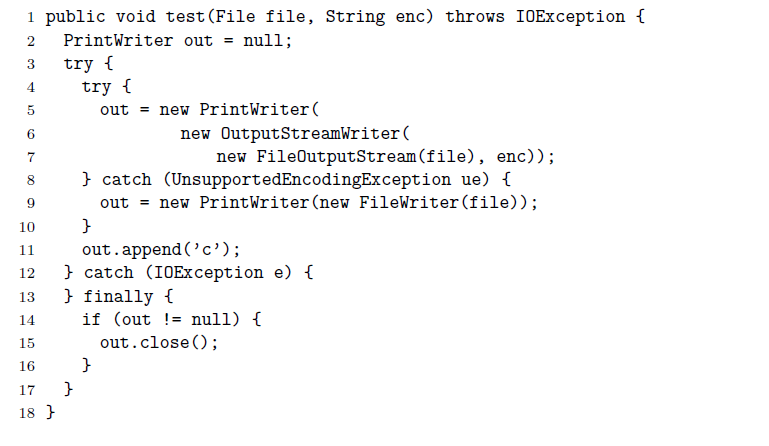
\includegraphics[width=\paperwidth]{fig1.png}
\end{frame}

\begin{frame}{Two Alias Analysis Characteristics}
	\begin{block}{Flow-sensitivity}
		Flow-sensitive analysis computes aliases for all flow paths in the program, while flow-insensitive
		analysis computes aliasing for the program as a whole.
	\end{block}
	\pause
	\begin{block}{Context-sensitivity}
		Context-sensitivity is about function/procedure calls and means whether a context of a call is taken
		into consideration or not.
	\end{block}
\end{frame}

\section{Points-To Analysis}

\subsection{Formulation}

\begin{frame}{Point-to Analysis}
	\begin{block}{}
		Paper presents several common variants of Andersen's point-to analysis.
	\end{block}
	\pause
	\begin{block}{Point-to analysis}
		A points-to analysis computes an over-approximation of the heap locations that
		each program pointer may point to. Pointers include program variables and also
		pointers within heap-allocated objects, e.g., instance fields. 
	\end{block}
	\pause
	\begin{block}{}
		The result of the analysis is a points-to relation pt, with pt(p) representing 
		the points-to set of a pointer p.
	\end{block}
	\pause
	\begin{block}{}
		Point-to analysis is flow insensitive: it assumes statements can execute in any order
		and any number of times.
	\end{block}	
\end{frame}

\begin{frame}{Point-to Analysis Statements}
	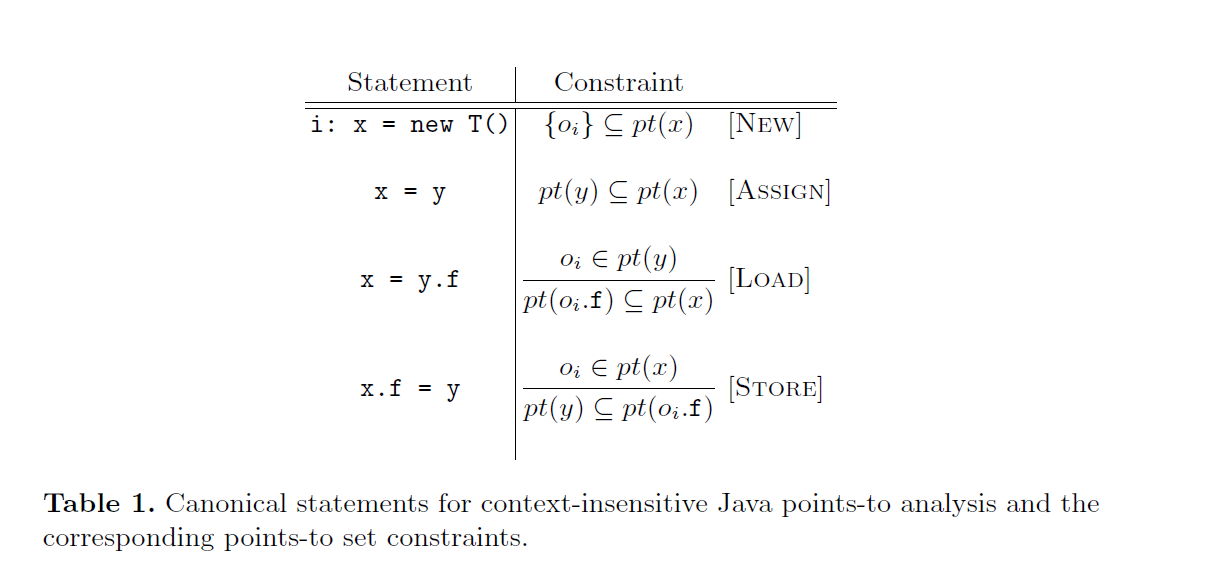
\includegraphics[width=\paperwidth]{table1.png}
\end{frame}

\begin{frame}{Context Sensitivity}
	\begin{block}{Context sensitivity}
		It is possible to extend point-to analysis to incorporate context-sensitive handling of method calls. 
	\end{block}
	\pause
	\begin{block}{}
		A context-sensitive points-to analysis separately analyzes a method m for
		each calling context that arises at call sites of m. 
	\end{block}
	\pause
	\begin{block}{}
		Separately analyzing a method for each context removes imprecision due to
		the merge of analysis results across its invocations.
	\end{block}
	\pause
	\centerline{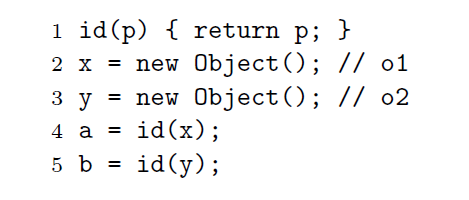
\includegraphics[width=0.5\paperwidth]{fig2.png}}
\end{frame}

\begin{frame}{Point-to Analysis Context-sensitive Statements}
	\centerline{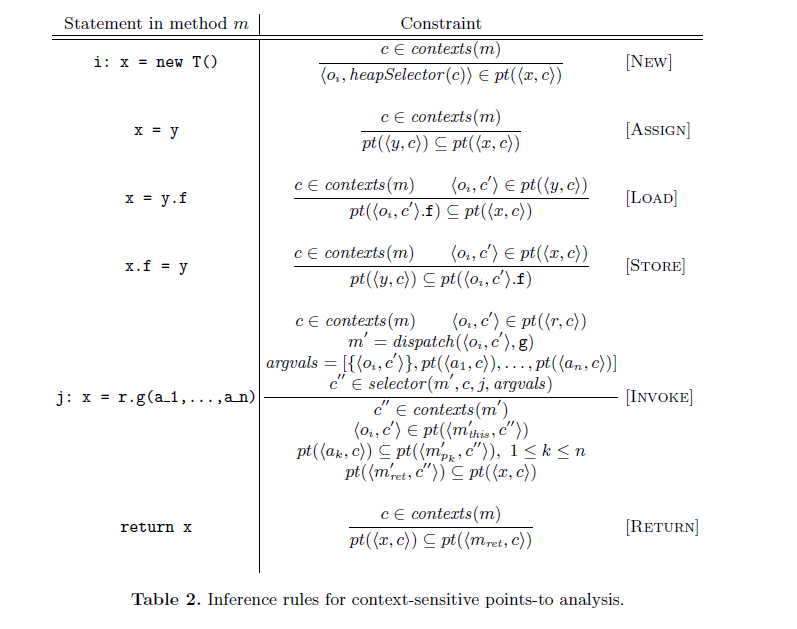
\includegraphics[width=0.8\paperwidth]{table2.png}}
\end{frame}

\begin{frame}{Context Sensitivity Variants}
	\begin{block}{Call strings}
		A standard technique to distinguish contexts is via \textit{call strings}, which abstract the possible call
		stacks under which a method may be invoked. Call strings are typically represented as
		a sequence of call site identifiers, corresponding to a (partial) call stack.
	\end{block}
	\pause
	\begin{block}{}
		Call string are often k-limited (only first k call site identifiers are considered).
	\end{block}
	\pause
	\begin{block}{Object sensitivity}
		Technique to distinguish contexts via objects which invoke methods.
	\end{block}
	\pause
	\begin{block}{}
		And there many more approaches and variants to distinguish contexts.
	\end{block}
\end{frame}

\subsection{Implementation}

\begin{frame}{Algorithm}
	\begin{block}{Algorithm}
		Algorithm, implementing Andersen's context-insensitive ponts-to analysis, constructs a flow graph 
		$G$ representing the pointer flow for a program.
	\end{block}
	\pause
	\begin{block}{}
		$G$ has nodes for variables, abstract locations, and field of abstract locations. 
	\end{block}
	\pause
	\begin{block}{}
		$G$ has an edge $n \rightarrow n'$ iff one of the following two conditions holds:
		\setbeamertemplate{enumerate items}[default]
		\begin{enumerate}
   			\item $n$ is an abstract location $o_i$ representing a statement x = new T(), and $n'$
   			is x.
   			\item $pt(n) \subseteq pt(n')$ according to some rule.
		\end{enumerate}
	\end{block}
\end{frame}

\begin{frame}{Algorithm Pseudocode}
	\centerline{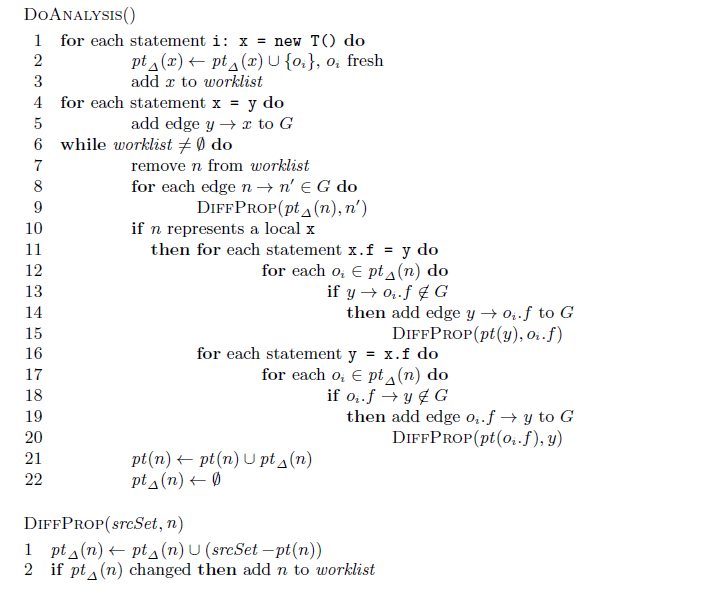
\includegraphics[width=0.75\paperwidth]{fig3.png}}
\end{frame}

\begin{frame}{Complexity}
	\begin{block}{Complexity}
		Algorithm from the previous slide has worst-case cubic complexity.
	\end{block}
	\pause
	\begin{block}{}
		In practice, many papers have reported scaling behavior significantly better
		than cubic (papers reporting analysis of millions of lines of code are now commonplace).
	\end{block}
\end{frame}

\begin{frame}{Optimizations}
	\begin{block}{Type filters}
		Algorithm from the previous slide has worst-case cubic complexity.In strongly-typed languages, type 
		filters provide a simple but highly effective optimization which improves 
		both precision and (usually) performance.
	\end{block}
	\pause
	\begin{block}{Cycle elimination}
		Collapse cycles in the flow graph.
	\end{block}
	\pause
	\begin{block}{Method-local state}
		If a variable's points-to set is determined entirely by statements in the enclosing method,
		the points-to set is computed on-demand rather than via the global constraint system.
	\end{block}
\end{frame}

\begin{frame}{Other Directions}
	\begin{block}{Context sensitivity}
		The most straightforward strategy for implementing context sensitivity
		is via \textit{cloning}.
	\end{block}
	\pause
	\begin{block}{}
		There are also many other strategies and solutions usually relying on clever data structures.
	\end{block}
	\pause
	\begin{block}{Demand-driven analysis}
		The previous discussion focused on computing an \textit{exhaustive} points-to analysis
		solution, i.e., computing all points-to sets for a program.
	\end{block}
	\pause
	\begin{block}{}
		However, this is usually not required in practice.
	\end{block}
\end{frame}

\section{Must-Alias Analysis}

\begin{frame}{Must-Alias Analysis}
	\begin{block}{Must-alias analysis}
		Paper presents a flow-sensitive must-alias analysis based on \textit{access paths}
	\end{block}
	\pause
	\begin{block}{}
		Must-alias analysis provides information about whether two pointers must be
		aliased at some program point.
	\end{block}
\end{frame}

\begin{frame}{Must-Alias Analysis Importance}
	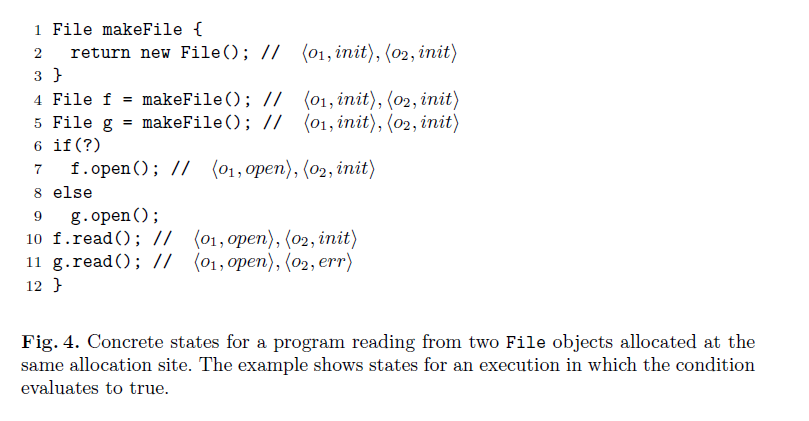
\includegraphics[width=\paperwidth]{fig4.png}
\end{frame}

\begin{frame}{May-Alias Analysis Drawback}
	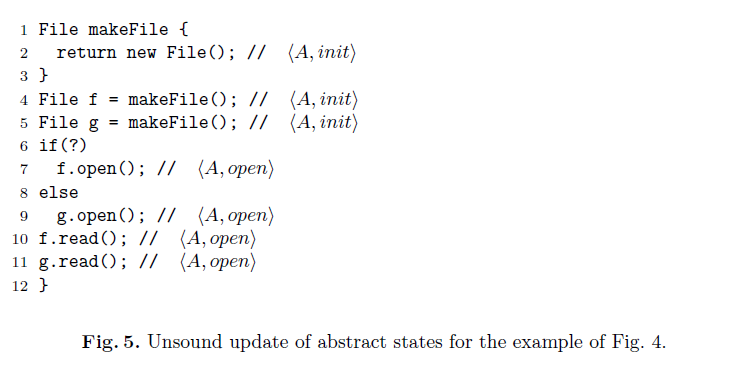
\includegraphics[width=\paperwidth]{fig5.png}
\end{frame}

\begin{frame}{Weak Updates}
	\begin{block}{Weak update}
		Weak update reflects all possible states of an object.
		\newline
		However, this fails even in simple cases.
	\end{block}
	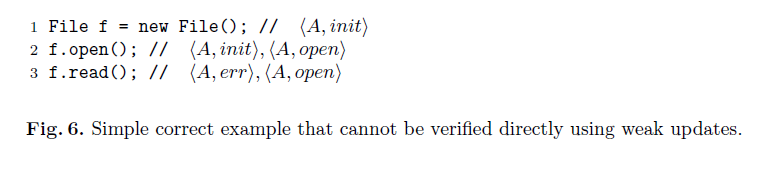
\includegraphics[width=0.9\paperwidth]{fig6.png}
	\begin{block}{Must-alias information}
		Correct analysis of this requires must-alias information
	\end{block}
\end{frame}

\begin{frame}{Access Paths}
	\begin{block}{Access path}
		Must-alias information is maintained with a help of \textit{access paths} --- a sequences of references
		that point to a heap allocated object. 
	\end{block}
\end{frame}

\begin{frame}{Maintaining Must Points-to Information}
	\begin{block}{}
		To describe the abstraction, first assume that a preliminary 
		flow-insensitive points-to analysis has run.
	\end{block}	
	\pause
	\begin{block}{Aliasing relationships in the form of tuples}
		We represent aliasing relationships with tuples of the form $\langle o, unique, AP_m, May, AP_{mn}
		\rangle$ where:
		\newline
		- $o$ is an instance key (abstract memory location from the preliminary points-to analysis).
		\newline
		- $unique$ indicates whether the corresponding allocation site has a single concrete
		live object.
		\newline
		- $AP_m$ is a set of access paths that must point-to $o$.
		\newline
		- $May$ is a boolean that indicates whether there are access paths (not in the
		must set) that may point to $o$.
		\newline
		- $AP_{mn}$ is a set of access paths that do not point-to $o$.
	\end{block}
\end{frame}

\begin{frame}{Tuple Transformers}
	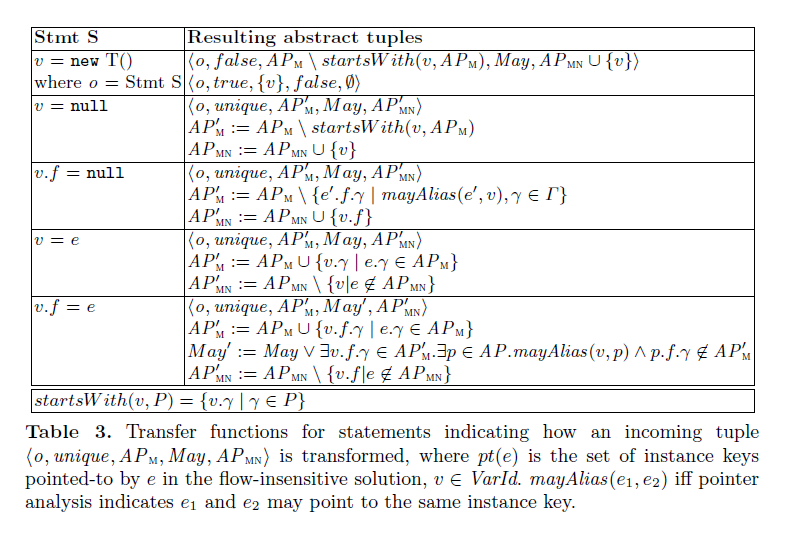
\includegraphics[width=0.9\paperwidth]{table3.png}
\end{frame}

\begin{frame}{Strong Updates with Access Paths}
	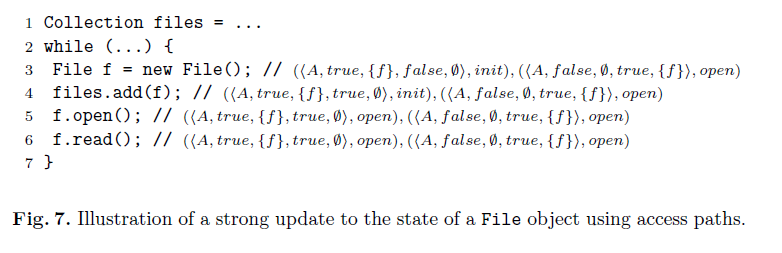
\includegraphics[width=\paperwidth]{fig7.png}
\end{frame}

\section{Analyzing Modern Java Programs}

\begin{frame}{Points-to Analysis Difficulties}
	\begin{block}{Reflection}
		In Java-like languages, reflection allows for meta-programming based on string
		names of program constructs like classes or methods.
	\end{block}	
	\pause
	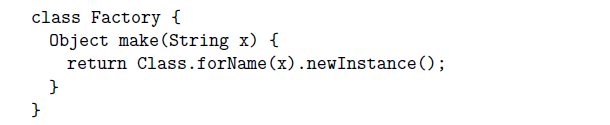
\includegraphics[width=\paperwidth]{fig8.png}
	\pause
	\begin{block}{}
		Analyzing this code with the assumption that x may name any type yields
		extremely imprecise results.
	\end{block}	
	\pause
	\begin{block}{Libraries and frameworks}
		Also, usage of large number of libraries and frameworks (with many of them using reflection) makes 
		analysis much more difficult.
	\end{block}	
\end{frame}

\begin{frame}{Under-Approximate Techniques}
	\begin{block}{Under-approximate techniques}
		Possible solution of problems of Java-like languages. 
	\end{block}	
	\pause
	\begin{block}{}
		Uses simpler versions of access path method, or some other domain-specific techniques.
		In general produces less accurate and sound result.
	\end{block}	
\end{frame}

\section{Conclusion}

\begin{frame}{Conclusion}
	\begin{block}{Conclusion}
		Paper have presented a high-level overview of state-of-the-art may- and must-alias
		analyses for object-oriented programs, based on authors' experiences implementing
		production-quality static analyses for Java. The sound alias-analysis techniques
		presented there work well for medium-sized programs, while for large-scale Java
		programs, an under-approximate alias analysis based on access-path tracking
		currently yields the most useful results.
	\end{block}	
\end{frame}

\begin{frame}{Future Work}
	\begin{block}{}
		Potentially fruitful directions for future work:
	\end{block}	
	\pause	
	\begin{block}{Reflection}
		Solution of reflection problem for Java-like languages
	\end{block}	
	\pause	
	\begin{block}{Dynamically-Typed Languages}
		Analysis of languages like JavaScript.
	\end{block}	
	\pause	
	\begin{block}{Developer Tool Integration}
		Integrate alias analysis with some developer tools.
	\end{block}	
\end{frame}

\begin{frame}{}
	\begin{spacing}{1.5}
		\LARGE{\centerline{Thank you for attention}}
	\end{spacing}
	\large{\centerline{Questions?}}
\end{frame}

\begin{frame}{References}
	\setbeamertemplate{enumerate items}[default]
	\begin{enumerate}
   		\item Alias analysis for object-oriented programs (by M. Sridharan, S. Chandra, J. Dolby, S.J. Fink,
   		 and E. Yahav, Lecture Notes in Computer Science, 2013, Vol. 7850, p. 196-232.)
   		\item Alias Calculus for a Simple Imperative Language with Decidable Pointer Arithmetic (Nikolay
   		 Shilov, Aizhan Satekbayeva, Aleksandr P. Vorontsov)
	\end{enumerate}
\end{frame}

\end{document}